\section{Udviklingsforløb}
I dette afsnit vil metoderne, der er blevet brugt i projektet, blive forklaret, hvordan disse er blevet benyttet og deres bidrag til projektet.

\subsection{ASE-modellen} \label{sec:ASEModel}
Den udviklingsmodel, som primært er brugt i projektet, er ASE modellen, som ses på figur \ref{fig:ASE}. ASE modellen \cite{ASE} er en mellemvægtig semi-iterativ udviklingsmodel, som er drevet ud fra en kravspecifikation, der bygger på user stories. ASE modellen tager udgangspunkt i vandfaldsmodellen til at opbygge dit projekt gennem faserne: Projektformulering - Kravspecifikation - Systemarkitektur -  Implementering -  Test/fejlfinding -  Integration og vedligeholdelse\cite{ASE}.

\begin{figure} [H]
	\begin{center}
		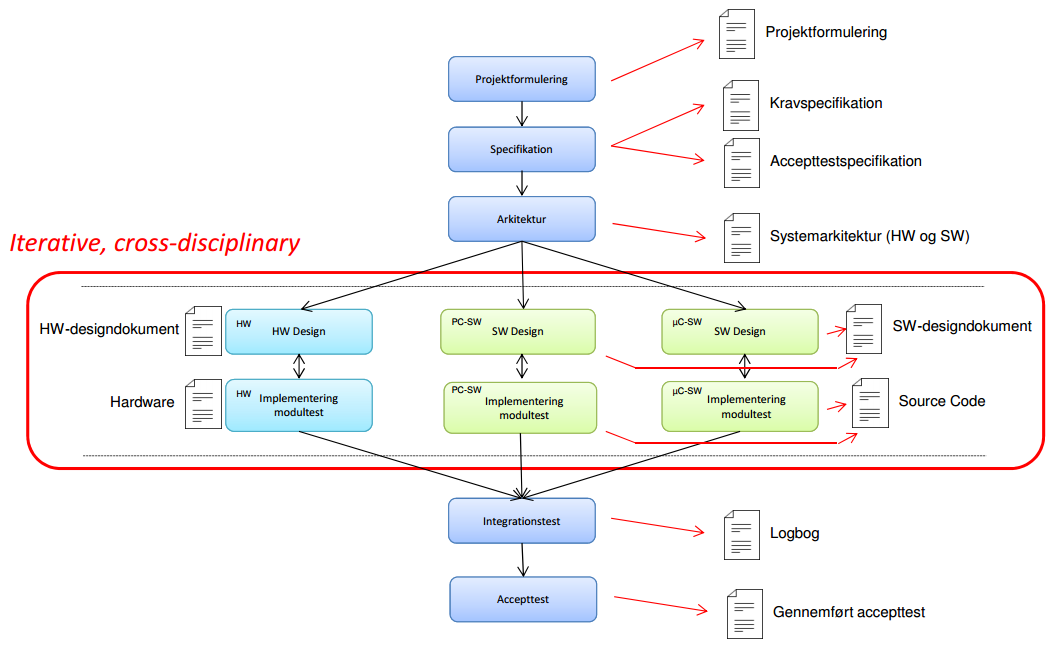
\includegraphics[height=10cm, width=12cm]{Udviklingsforlob/ASEModellen}
	\end{center}
	\caption{ASE modellen. \cite{ASE}}
	\label{fig:ASE}
\end{figure}

Første punkt i ASE modellen er, at få skrevet en projektformulering og herefter en kravspecifikation, som består af en række user stories. User stories er et værktøj, der beskriver, hvordan der interageres med systemet. Efterfølgende opbygges en kravspecifikation ud fra user stories, og herved opnås et godt overblik over, hvilke krav der er til systemet. Accepttesten specificeres derefter ud fra kravspecifikationen, så alle dele i det samlede system bliver testet.
Der er tilføjet en analyse til modellen for at kunne redegøre for de valg, der er taget i projektet. Analysen blev udarbejdet sideløbende med kravspecifikationen. \\
Når kravspecifikationen er udarbejdet, påbegyndes udarbejdningen af systemarkitekturen. I systemarkitekturen skematiseres systemets moduler og grænseflader til de andre moduler i systemet. Når den overordnede arkitektur er på plads, brydes systemet op efter funktionalitet. \\
I design- og implementeringsfaserne er der anvendt en iterativ proces. Dette har gjort udviklingen mere fleksibel. \\

\subsection{Scrum}
Scrum \cite{Scrum} er en agil udviklingsproces med fokus på projektledelse. Forskellen på Scrum og andre arbejdsmetoder som f.eks. vandfaldmodellen\cite{Vandfald} er, at Scrum er en iterativ proces og ikke en lineær proces.

Scrum er bygget op omkring roller; Scrum Master, Product Owner og Development Team. Product Owner'en er ansvarlig for produktet og for product backlog'en, som indeholder alt det arbejde, der mangler at blive lavet\cite{Scrum}. \\
Scrum Master'en er ansvarlig for at Development team'et performer optimalt og fjerne unødvendige forstyrrelser under udviklingsprocessen. \\
Development team'et er udviklingsteamet, som står for at udføre de opgaver, som Product Owner'en tager fra backlog'en og tilfører de enkelte sprints. \\
I dette projekt var hele gruppen både Development Team og Product Owner. Morten agerede Scrum Master gennem hele projektet og stod bl.a. også for kommunikationen til Rambøll og vejlederen. \\



